```latex
% Fashion Tech Pack LaTeX Template - Updated with TechPack.ai in Corner and Aligned Technical Specs
\documentclass[11pt,a4paper]{article}

% Required packages
\usepackage[utf8]{inputenc}
\usepackage[T1]{fontenc}
\usepackage{lmodern}
\usepackage[english]{babel}
\usepackage{xcolor}
\usepackage{graphicx}
\usepackage{tabularx}
\usepackage{booktabs}
\usepackage{array}
\usepackage{colortbl}
\usepackage{multirow}
\usepackage{tikz}
\usepackage{tcolorbox}
\usepackage{enumitem}
\usepackage{fancyhdr}
\usepackage[hidelinks]{hyperref}
\usepackage{geometry}
\usepackage{pifont}
\usepackage{fontawesome5}
\usepackage{float}
\usepackage{pdflscape} % For landscape pages if needed
\usepackage{lipsum}

\graphicspath{{illustration/}{reference/}}  % DO NOT CHANGE THIS LINE

% Page geometry
\geometry{
  a4paper,
  top=1.5cm,
  bottom=2cm,
  left=1.5cm,
  right=1.5cm,
  footskip=1.5cm
}

% New color definitions for a modern headline
\definecolor{modernStart}{RGB}{30, 30, 70}  % dark blue
\definecolor{modernEnd}{RGB}{70, 100, 200}   % lighter blue

% Other color definitions
\definecolor{tableheader}{RGB}{220, 230, 242}
\definecolor{bordergray}{RGB}{180, 180, 180}
\definecolor{lightblue}{RGB}{221, 235, 247}
\definecolor{accentblue}{RGB}{0, 120, 200}

% Style settings
\setlength{\parindent}{0pt}
\setlength{\parskip}{0.5em}
\renewcommand{\arraystretch}{1.5}

% Header and footer
\pagestyle{fancy}
\fancyhf{}
\renewcommand{\headrulewidth}{0pt}

% 1) Tiny "TechPack.ai" in the upper left corner on every page
\fancyhead[L]{\tiny \textbf{TechPack.ai}}

% Footer
\fancyfoot[C]{\textcopyright\
  \ \textbf{\CompanyName} \the\year. All Rights Reserved.}
\fancyfoot[R]{\thepage}

% Custom commands for tech pack data
\newcommand{\CompanyName}{EK}
\newcommand{\StyleName}{Bomber Jacket}
\newcommand{\StyleNumber}{Jkt-03384}
\newcommand{\Designer}{William}
\newcommand{\Season}{Spring 2025}
\newcommand{\TechPackVersion}{V1}
\newcommand{\TechPackDate}{03/03/2025}
\newcommand{\Category}{Men's Outerwear}
\newcommand{\Finalized}{No}
\newcommand{\Approved}{No}

% Custom section header command (used on most pages)
\newcommand{\techsection}[1]{
  \vspace{0.8cm}
  \begin{tcolorbox}[
    enhanced,
    colback=accentblue!80,
    colframe=accentblue,
    coltext=white,
    round corners,
    boxrule=0pt,
    width=\textwidth,
    halign=left,
    fontupper=\large\bfseries,
    top=0.4cm,
    bottom=0.4cm,
    left=0.2cm,
    right=0.2cm
  ]
    #1
  \end{tcolorbox}
  \vspace{0.3cm}
}

% Custom command for image placeholders (replace {} with filename)
\newcommand{\imagebox}[2][6cm]{%
  \fbox{%
    \begin{minipage}[c][#1][c]{0.95\linewidth}%
      \centering%
      \ifx\relax#2\relax%
        \huge\textbf{Image\\Placeholder}%
      \else%
        \includegraphics[height=#1,width=\linewidth,keepaspectratio]{#2}%
      \fi%
    \end{minipage}%
  }%
}

\begin{document}

%% --- Title Page with Modern Gradient Headline ---
\begin{tcolorbox}[
  enhanced,
  width=\textwidth,
  halign=center,
  valign=center,
  height=1.2cm,
  round corners,
  boxrule=0pt,
  interior style={left color=modernStart, right color=modernEnd}
]
  \textcolor{gray}{\Large\bfseries TechPack.ai - Create tech packs in minutes, not hours}
\end{tcolorbox}

\vspace{1cm}
\begin{center}
  {\Huge\bfseries Technical Specification Sheet}
\end{center}
\vspace{1cm}

%%%%%%%%%%%%%%%%%%%%%%%%%%%%%%%%%%%%%%%%%%%%
% Page 1: Basic Info, Sketches, and Revision History
%%%%%%%%%%%%%%%%%%%%%%%%%%%%%%%%%%%%%%%%%%%%

% Re-designed Basic Information Table: 4 columns x 5 rows
\begin{table}[H]
  \centering
  \resizebox{\linewidth}{!}{%
  \begin{tabular}{|p{3cm}|p{3.5cm}|p{3cm}|p{3.5cm}|}
    \hline
    \textbf{Brand:} & \CompanyName & \textbf{Designer:} & \Designer \\
    \hline
    \textbf{Style Name:} & \StyleName & \textbf{Style Number:} & \StyleNumber \\
    \hline
    \textbf{Category:} & \Category & \textbf{Season:} & \Season \\
    \hline
    \textbf{Date:} & \TechPackDate & \textbf{Version:} & \TechPackVersion \\
    \hline
    \textbf{Finalized:} & \Finalized & \textbf{Approved:} & \Approved \\
    \hline
  \end{tabular}%
  }
\end{table}

\vspace{0.5cm}
% Directly beneath: Sketches (two images side by side; no headline)
\begin{table}[H]
  \centering
  \begin{tabular}{cc}
    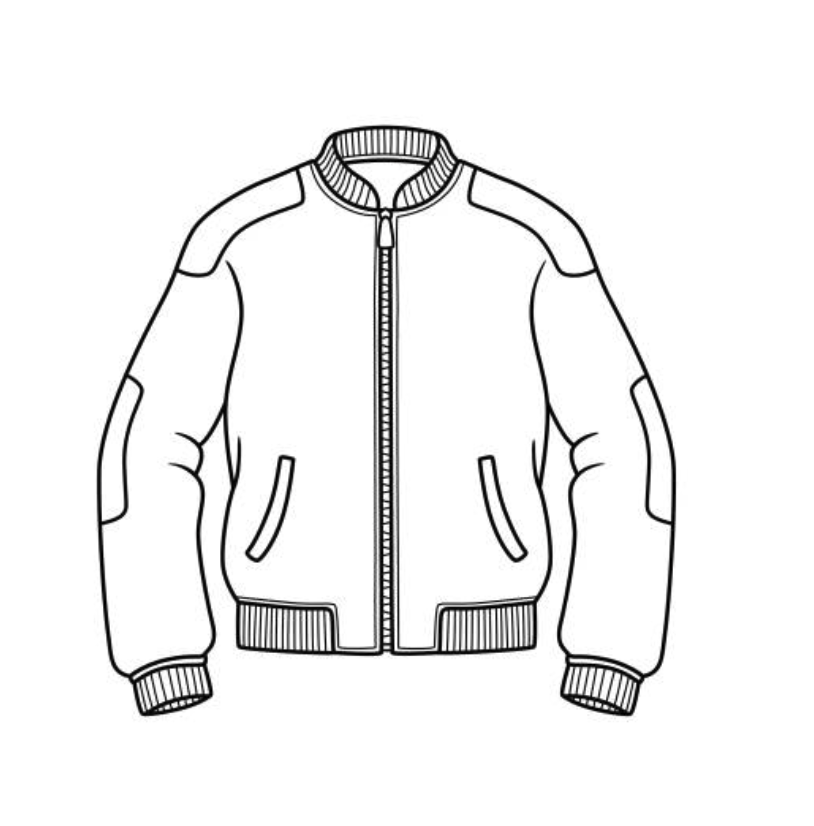
\includegraphics[width=0.48\linewidth]{Screenshot_2025-03-09_at_22.37.32.png} & \includegraphics[width=0.48\linewidth]{DALLE_2025-03-09_22.47.57_-_A_realistic_bomber_jacket_in_a_neutral_color_shown_from_the_front_view._The_jacket_has_a_ribbed_collar_1.5_inches_tall_full-length_zipper_22_inch.webp} \\
    \small Illustration & \small Front Reference \\
  \end{tabular}
\end{table}

\vspace{0.5cm}
% Revision History table on the same page
\begin{table}[H]
  \centering
  \resizebox{\linewidth}{!}{%
  \begin{tabular}{|p{2cm}|p{12cm}|}
    \hline
    \rowcolor{tableheader}
    \textbf{Version} & \textbf{Description} \\
    \hline
    V1 & This is the first draft \\
    \hline
    V2 & \\
    \hline
    V3 & \\
    \hline
  \end{tabular}%
  }
\end{table}

%%%%%%%%%%%%%%%%%%%%%%%%%%%%%%%%%%%%%%%%%%%%
% Page 2: Design Description
%%%%%%%%%%%%%%%%%%%%%%%%%%%%%%%%%%%%%%%%%%%%

\newpage
\techsection{General Design Description}
\begin{tcolorbox}[
  colback=white,
  colframe=accentblue,
  width=\textwidth,
  height=10cm,  % Adjust as needed
]
The design is a classic bomber jacket featuring a ribbed collar, cuffs, and waistband for a snug fit. It has a full-length zipper, welt pockets, and shoulder patches for added structure and style. The silhouette is slightly blouson, tapering at the waistband, with a clean back panel for a timeless design. The use of mid-weight nylon/polyester or cotton blend ensures durability and comfort.
\end{tcolorbox}

%%%%%%%%%%%%%%%%%%%%%%%%%%%%%%%%%%%%%%%%%%%%
% Page 3: Technical Specification - Front
%%%%%%%%%%%%%%%%%%%%%%%%%%%%%%%%%%%%%%%%%%%%

\techsection{Technical Specification - Front}

\begin{table}[H]
\centering
\begin{tabular}{@{}l l@{}}
\begin{minipage}[t]{0.5\linewidth}
  \vspace{0pt} % ensure top alignment
  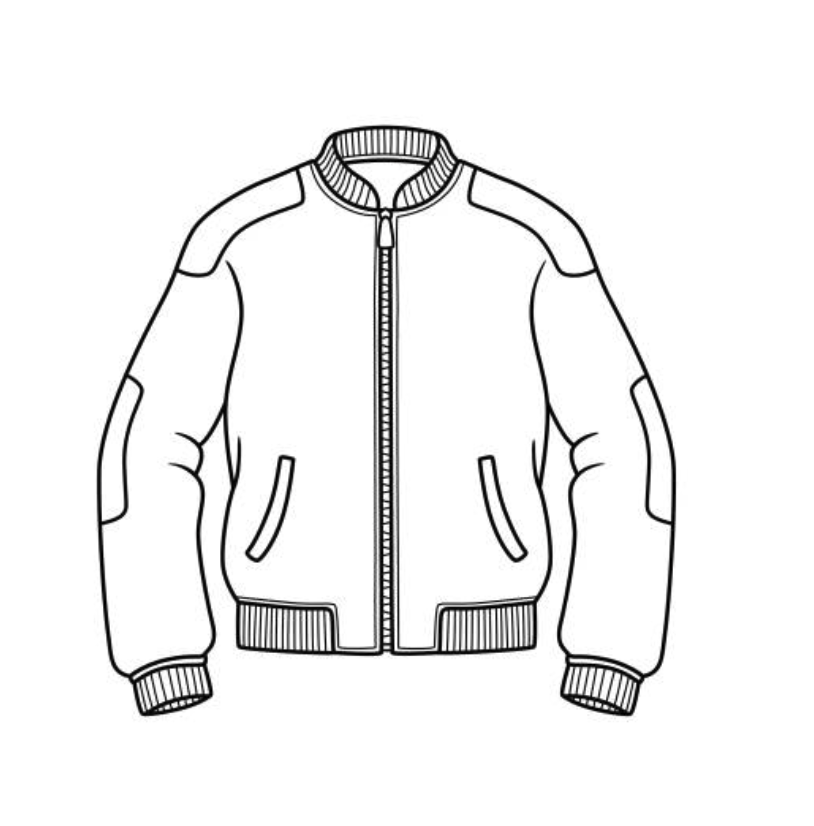
\includegraphics[width=\linewidth]{Screenshot_2025-03-09_at_22.37.32.png}
\end{minipage}
&
\begin{minipage}[t]{0.5\linewidth}
  \vspace{0pt} % ensure top alignment
  \begin{tabular}{|c|p{0.85\linewidth}|}
    \hline
    \textbf{1} & Ribbed collar, 1.5 inches (3.8 cm) height \\ \hline
    \textbf{2} & Full-length zipper, 22 inches (56 cm) \\ \hline
    \textbf{3} & Two main front panels \\ \hline
    \textbf{4} & Welt pockets, 6 inches (15 cm) wide \\ \hline
    \textbf{5} & Shoulder panels, 6 inches (15 cm) long \\ \hline
  \end{tabular}
\end{minipage}
\end{tabular}
\end{table}

%%%%%%%%%%%%%%%%%%%%%%%%%%%%%%%%%%%%%%%%%%%%
% Page 4: Technical Specification - Back
%%%%%%%%%%%%%%%%%%%%%%%%%%%%%%%%%%%%%%%%%%%%

\techsection{Technical Specification - Back}

\begin{table}[H]
\centering
\begin{tabular}{@{}l l@{}}
\begin{minipage}[t]{0.5\linewidth}
  \vspace{0pt}
  \includegraphics[width=\linewidth]{DALLE_2025-03-09_22.47.56_-_A_realistic_bomber_jacket_in_a_neutral_color_shown_from_the_side_view._The_jacket_features_a_ribbed_collar_full-length_zipper_in_the_front_and_a_sl.webp}
\end{minipage}
&
\begin{minipage}[t]{0.5\linewidth}
  \vspace{0pt}
  \begin{tabular}{|c|p{0.85\linewidth}|}
    \hline
    \textbf{1} & Single main back panel \\ \hline
    \textbf{2} & Shoulder patch continuation \\ \hline
    \textbf{3} & Back yoke, 2 inches (5 cm) below collar \\ \hline
    \textbf{4} & Ribbed waist, 2.5 inches (6.4 cm) height \\ \hline
  \end{tabular}
\end{minipage}
\end{tabular}
\end{table}

%%%%%%%%%%%%%%%%%%%%%%%%%%%%%%%%%%%%%%%%%%%%
% Page 5: Lookalike
%%%%%%%%%%%%%%%%%%%%%%%%%%%%%%%%%%%%%%%%%%%%

\newpage
\techsection{Lookalike}
% Upper part: two images side by side for lookalike references
\begin{table}[H]
  \centering
  \begin{tabular}{cc}
    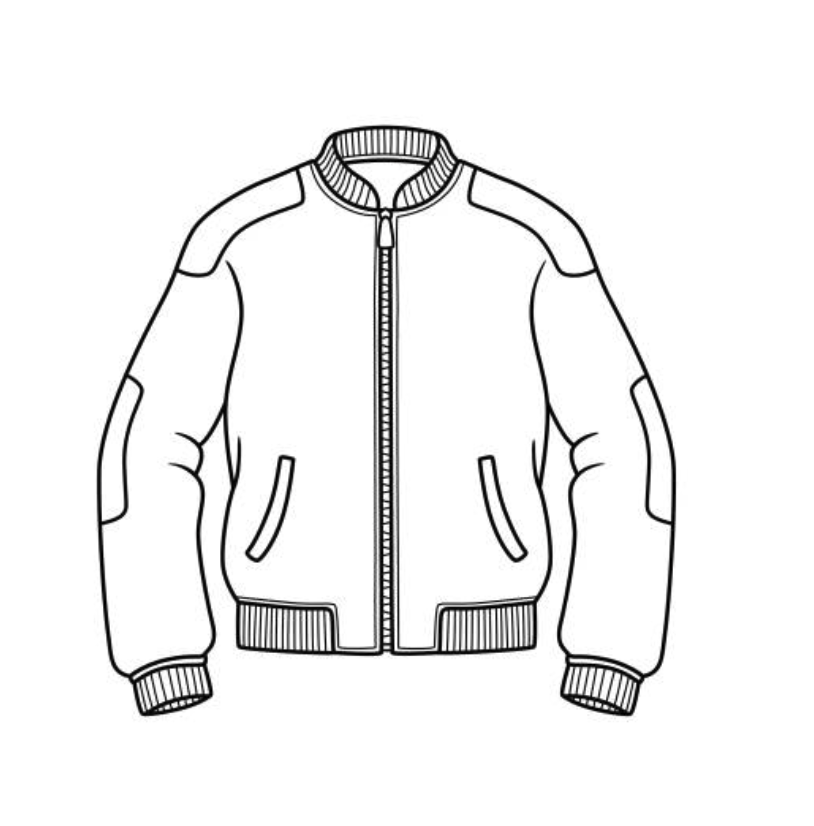
\includegraphics[width=0.45\linewidth]{Screenshot_2025-03-09_at_22.37.32.png} & \includegraphics[width=0.45\linewidth]{DALLE_2025-03-09_22.47.57_-_A_realistic_bomber_jacket_in_a_neutral_color_shown_from_the_front_view._The_jacket_has_a_ribbed_collar_1.5_inches_tall_full-length_zipper_22_inch.webp} \\
    \small Front Look & \small Side Look \\
  \end{tabular}
\end{table}

\vspace{1cm}
% Lower part: two description textboxes for designer comments
\begin{table}[H]
  \centering
  \begin{tabular}{cc}
    \begin{tcolorbox}[colback=white, colframe=accentblue, width=0.45\linewidth, title=Description, height=10cm]
      The front look showcases the classic bomber design with practical welt pockets and a robust full-length zipper.
    \end{tcolorbox}
    &
    \begin{tcolorbox}[colback=white, colframe=accentblue, width=0.45\linewidth, title=Description, height=10cm]
      The side view highlights the jacket's slightly blouson silhouette, offering a modern and comfortable fit.
    \end{tcolorbox}
  \end{tabular}
\end{table}

%%%%%%%%%%%%%%%%%%%%%%%%%%%%%%%%%%%%%%%%%%%%
% Page 6: Stitches
%%%%%%%%%%%%%%%%%%%%%%%%%%%%%%%%%%%%%%%%%%%%

\newpage
\techsection{Stitches}
% Upper part: two images side by side for design references
\begin{table}[H]
  \centering
  \begin{tabular}{cc}
    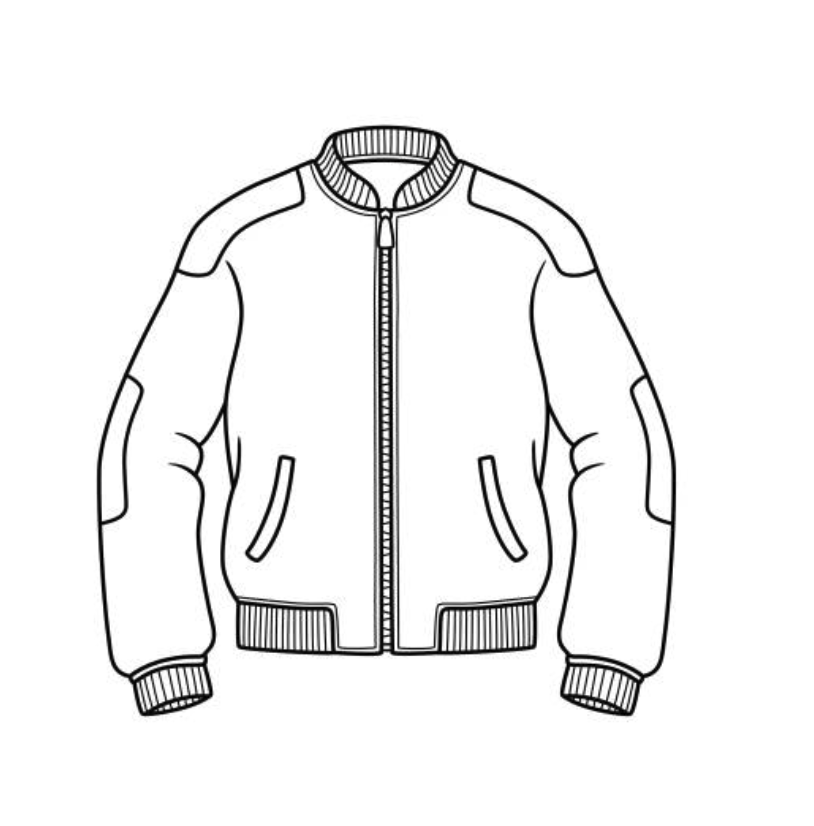
\includegraphics[width=0.45\linewidth]{Screenshot_2025-03-09_at_22.37.32.png} & \includegraphics[width=0.45\linewidth]{DALLE_2025-03-09_22.47.56_-_A_realistic_bomber_jacket_in_a_neutral_color_shown_from_the_side_view._The_jacket_features_a_ribbed_collar_full-length_zipper_in_the_front_and_a_sl.webp} \\
    \small Front Design & \small Side Design \\
  \end{tabular}
\end{table}

\vspace{1cm}
% Lower part: the existing stitches table (unchanged)
\begin{table}[H]
  \centering
  \resizebox{\linewidth}{!}{%
    \begin{tabular}{|p{1cm}|p{4cm}|p{3cm}|p{2.5cm}|p{2cm}|p{3.5cm}|}
      \hline
      \rowcolor{tableheader}
      \textbf{\#} & \textbf{Operation} & \textbf{Stitches} & \textbf{Width} & \textbf{SPI} & \textbf{Seams} \\
      \hline
      A & Seam joining the shoulder panels & Overlock & 1.5 cm & 10 & Flat seam \\
      \hline
      B & Pocket attachment & Coverstitch & 1 cm & 8 & Single seam \\
      \hline
      C & Cuffs and hem & Ribbed stitch & 4 cm & 12 & Double seam \\
      \hline
      D & Side seam & Overlock & 2 cm & 10 & Invisible seam \\
      \hline
    \end{tabular}%
  }
\end{table}

%%%%%%%%%%%%%%%%%%%%%%%%%%%%%%%%%%%%%%%%%%%%
% Page 7: Fabrics, Threads & Other
%%%%%%%%%%%%%%%%%%%%%%%%%%%%%%%%%%%%%%%%%%%%

\newpage
\techsection{Fabrics}
\begin{table}[H]
  \centering
  \resizebox{\linewidth}{!}{%
  \begin{tabular}{|p{2.5cm}|p{4cm}|p{2.5cm}|p{2.5cm}|p{2.5cm}|p{2cm}|}
    \hline
    \rowcolor{tableheader}
    \textbf{Item} & \textbf{Description} & \textbf{Image} & \textbf{Color} & \textbf{Color Code} & \textbf{Quantity} \\
    \hline
    Main Fabric & Mid-weight nylon/polyester & \includegraphics[width=2cm]{DALLE_2025-03-09_22.47.57_-_A_realistic_bomber_jacket_in_a_neutral_color_shown_from_the_front_view._The_jacket_has_a_ribbed_collar_1.5_inches_tall_full-length_zipper_22_inch.webp} & Neutral & 1234 & 2.5m \\[0.8cm]
    \hline
    Ribbed Fabric & Cotton-polyester blend & 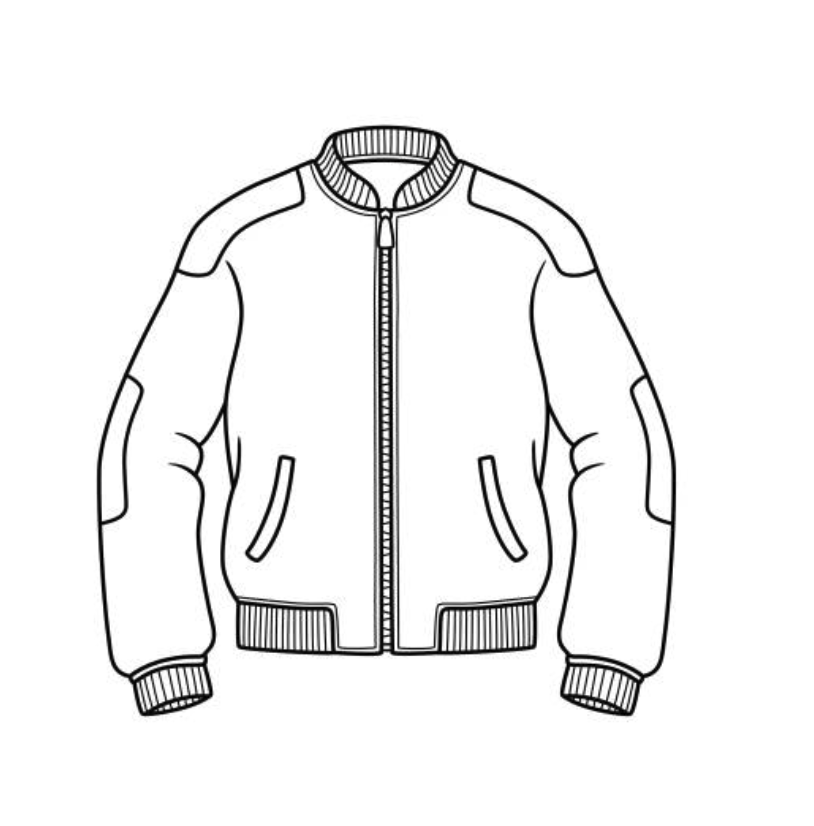
\includegraphics[width=2cm]{Screenshot_2025-03-09_at_22.37.32.png} & Neutral & 5678 & 1.0m \\[0.8cm]
    \hline
  \end{tabular}%
  }
\end{table}

\vspace{0.8cm}
\techsection{Threads}
\begin{table}[H]
  \centering
  \resizebox{\linewidth}{!}{%
  \begin{tabular}{|p{2.5cm}|p{4cm}|p{2.5cm}|p{2.5cm}|p{2.5cm}|p{2cm}|}
    \hline
    \rowcolor{tableheader}
    \textbf{Item} & \textbf{Description} & \textbf{Image} & \textbf{Color} & \textbf{Color Code} & \textbf{Quantity} \\
    \hline
    Top Threads & Polyester & 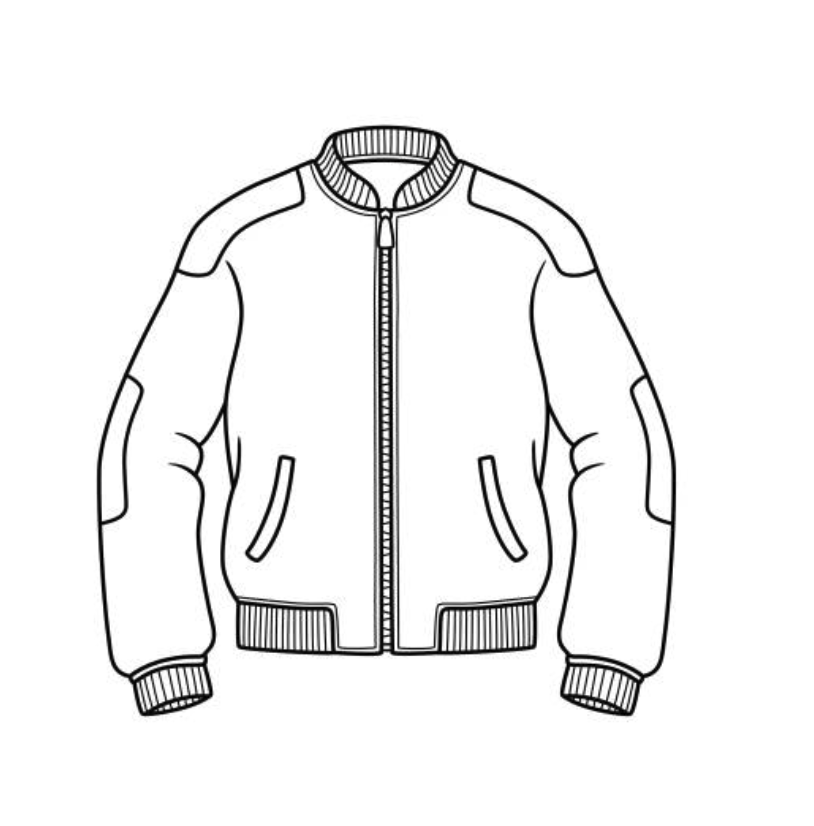
\includegraphics[width=2cm]{Screenshot_2025-03-09_at_22.37.32.png} & Neutral & 1234 & 200m \\[0.8cm]
    \hline
    Bottom Threads & Polyester & 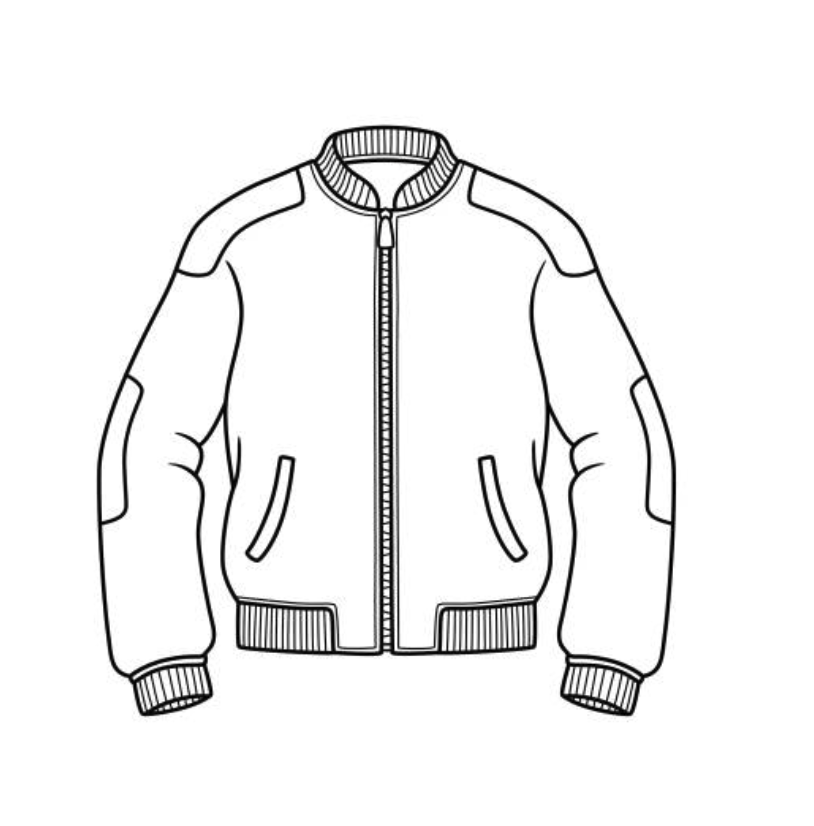
\includegraphics[width=2cm]{Screenshot_2025-03-09_at_22.37.32.png} & Neutral & 1234 & 200m \\[0.8cm]
    \hline
  \end{tabular}%
  }
\end{table}

\vspace{0.8cm}
\techsection{Other}
\begin{table}[H]
  \centering
  \resizebox{\linewidth}{!}{%
  \begin{tabular}{|p{2.5cm}|p{4cm}|p{2.5cm}|p{2.5cm}|p{2.5cm}|p{2cm}|}
    \hline
    \rowcolor{tableheader}
    \textbf{Item} & \textbf{Description} & \textbf{Image} & \textbf{Color} & \textbf{Color Code} & \textbf{Quantity} \\
    \hline
    Zipper & Metal zipper & 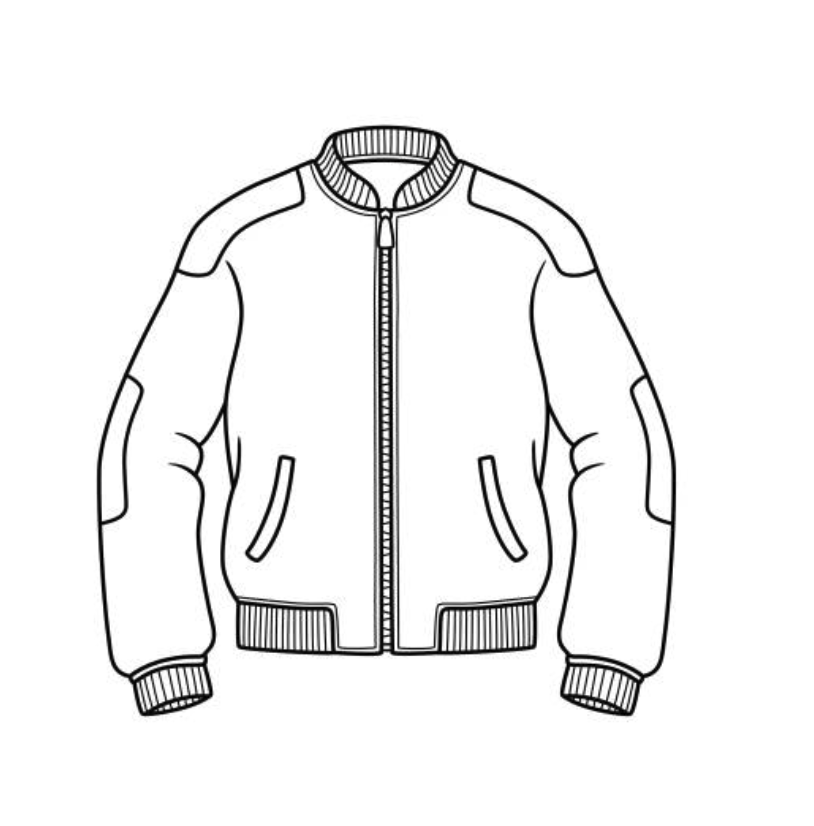
\includegraphics[width=2cm]{Screenshot_2025-03-09_at_22.37.32.png} & Silver & 9101 & 1 \\[0.8cm]
    \hline
  \end{tabular}%
  }
\end{table}

%%%%%%%%%%%%%%%%%%%%%%%%%%%%%%%%%%%%%%%%%%%%
% Page 8: Measurement Specifications
%%%%%%%%%%%%%%%%%%%%%%%%%%%%%%%%%%%%%%%%%%%%

\newpage
\techsection{Measurement Specifications}
\begin{table}[H]
  \centering
  \resizebox{\linewidth}{!}{%
    \begin{tabular}{|p{1.3cm}|p{5cm}|p{1.8cm}|p{1.8cm}|p{1.8cm}|p{1.8cm}|p{1.8cm}|p{1.8cm}|}
      \hline
      \rowcolor{lightblue}
      \textbf{POM} & \textbf{MEASUREMENT} & \textbf{XS} & \textbf{S} & \textbf{M} & \textbf{L} & \textbf{XL} & \textbf{TOL +/-} \\
      \hline
      A & Total Length & 67cm & 69cm & 71cm & 73cm & 75cm & 1cm \\
      \hline
      B & Chest Width & 56cm & 58cm & 60cm & 62cm & 64cm & 1cm \\
      \hline
      C & Body Width at Hem & 51cm & 53cm & 55cm & 57cm & 59cm & 1cm \\
      \hline
      D & Shoulder Width & 46cm & 48cm & 50cm & 52cm & 54cm & 1cm \\
      \hline
      E & Sleeve Length & 64cm & 65cm & 66cm & 67cm & 68cm & 1cm \\
      \hline
    \end{tabular}%
  }
\end{table}

%%%%%%%%%%%%%%%%%%%%%%%%%%%%%%%%%%%%%%%%%%%%
% Page 9: Colorways
%%%%%%%%%%%%%%%%%%%%%%%%%%%%%%%%%%%%%%%%%%%%

\newpage
\techsection{Colorways}
\begin{table}[H]
  \centering
  \resizebox{\linewidth}{!}{%
  \begin{tabular}{|p{3cm}|p{3.5cm}|p{2.5cm}|p{3cm}|p{2.5cm}|p{2.5cm}|}
    \hline
    \rowcolor{lightblue}
    \multicolumn{6}{|c|}{\textbf{Outside}} \\
    \hline
    \rowcolor{tableheader}
    \textbf{Area} & \textbf{Description} & \textbf{Color} & \textbf{Pantone Code} & \textbf{Image} & \textbf{Comments} \\
    \hline
    Main Body & Mid-weight fabric & Neutral & 1234 & \includegraphics[width=2cm]{DALLE_2025-03-09_22.47.57_-_A_realistic_bomber_jacket_in_a_neutral_color_shown_from_the_front_view._The_jacket_has_a_ribbed_collar_1.5_inches_tall_full-length_zipper_22_inch.webp} & Classic look \\[1cm]
    \hline
    Ribbing & Cotton-poly blend & Neutral & 5678 & 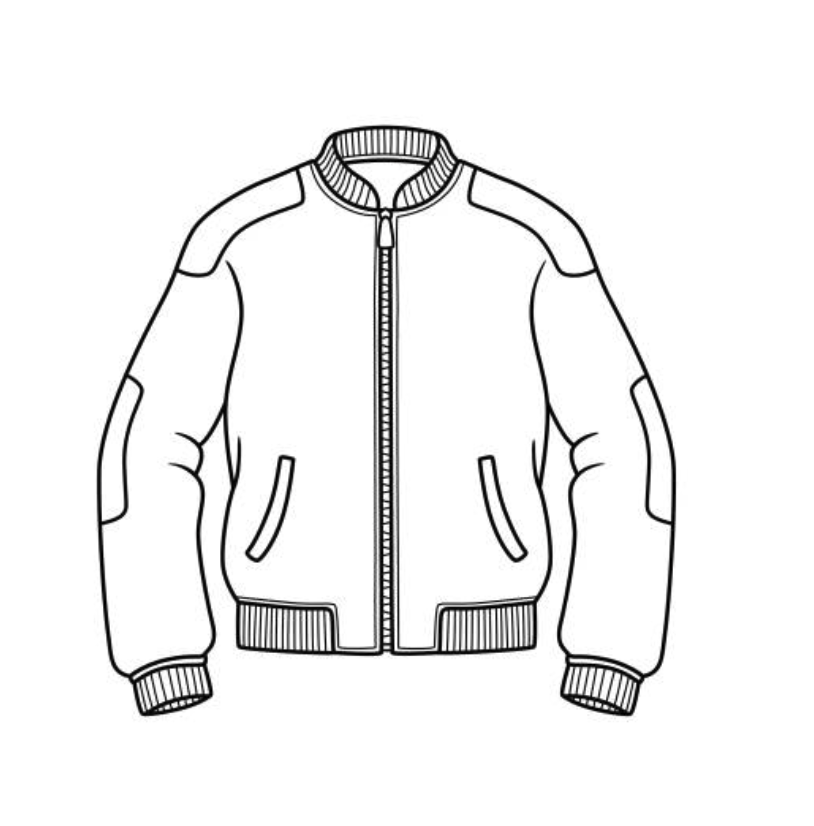
\includegraphics[width=2cm]{Screenshot_2025-03-09_at_22.37.32.png} & For collar, cuffs \\[1cm]
    \hline
  \end{tabular}%
  }
\end{table}

\vspace{0.8cm}
\begin{table}[H]
  \centering
  \resizebox{\linewidth}{!}{%
  \begin{tabular}{|p{3cm}|p{3.5cm}|p{2.5cm}|p{3cm}|p{2.5cm}|p{2.5cm}|}
    \hline
    \rowcolor{lightblue}
    \multicolumn{6}{|c|}{\textbf{Inside}} \\
    \hline
    \rowcolor{tableheader}
    \textbf{Area} & \textbf{Description} & \textbf{Color} & \textbf{Pantone Code} & \textbf{Image} & \textbf{Comments} \\
    \hline
    Lining & Soft touch fabric & Neutral & 5678 & 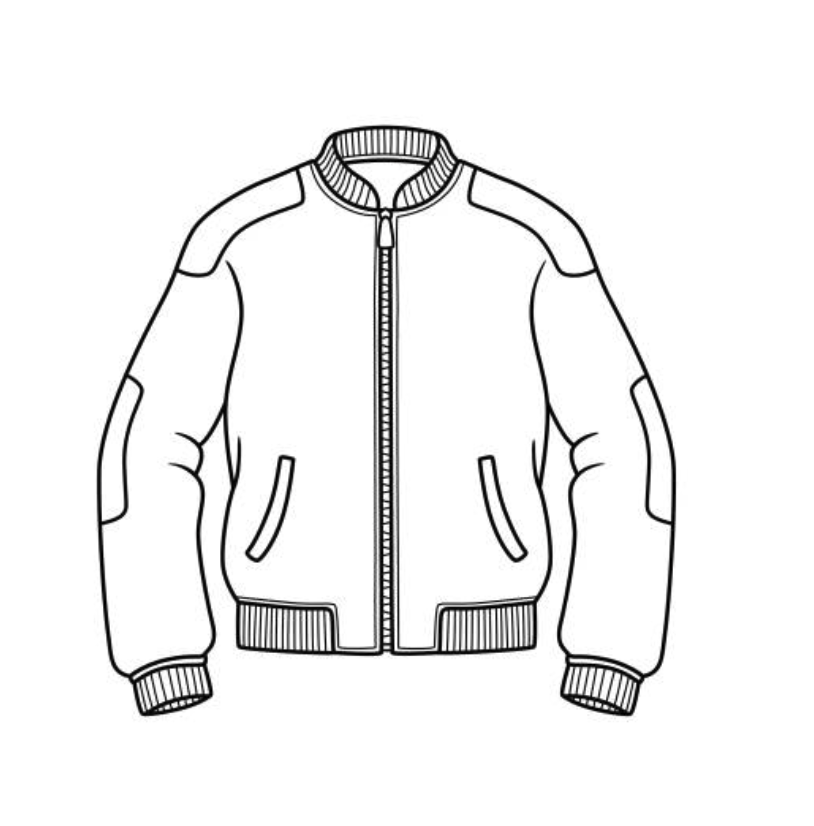
\includegraphics[width=2cm]{Screenshot_2025-03-09_at_22.37.32.png} & Comfortable wear \\[1cm]
    \hline
  \end{tabular}%
  }
\end{table}

%%%%%%%%%%%%%%%%%%%%%%%%%%%%%%%%%%%%%%%%%%%%
% Page 10: Label & Packaging
%%%%%%%%%%%%%%%%%%%%%%%%%%%%%%%%%%%%%%%%%%%%

\newpage
\techsection{Label}
\begin{table}[H]
  \centering
  \resizebox{\linewidth}{!}{%
  \begin{tabular}{|p{2.5cm}|p{4cm}|p{3cm}|p{2.5cm}|p{2cm}|p{2.5cm}|}
    \hline
    \rowcolor{tableheader}
    \textbf{Item} & \textbf{Description} & \textbf{Image} & \textbf{Color} & \textbf{Code} & \textbf{Quantity} \\
    \hline
    Brand Label & Embroidered logo & 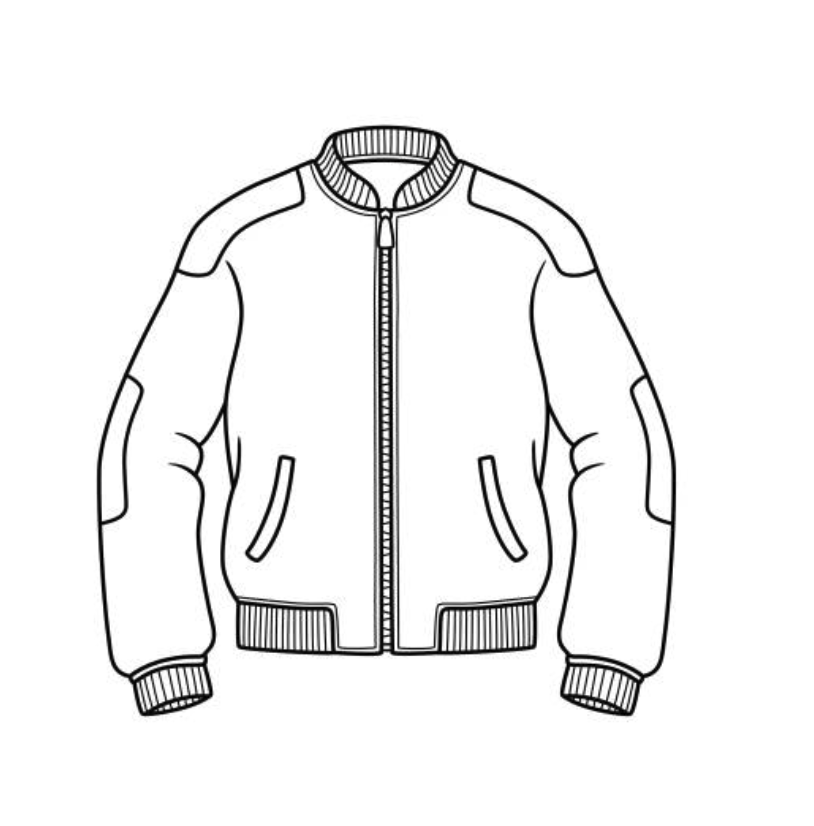
\includegraphics[width=2cm]{Screenshot_2025-03-09_at_22.37.32.png} & White & 3456 & 1 \\[1cm]
    \hline
    Care Label & Printed instructions & 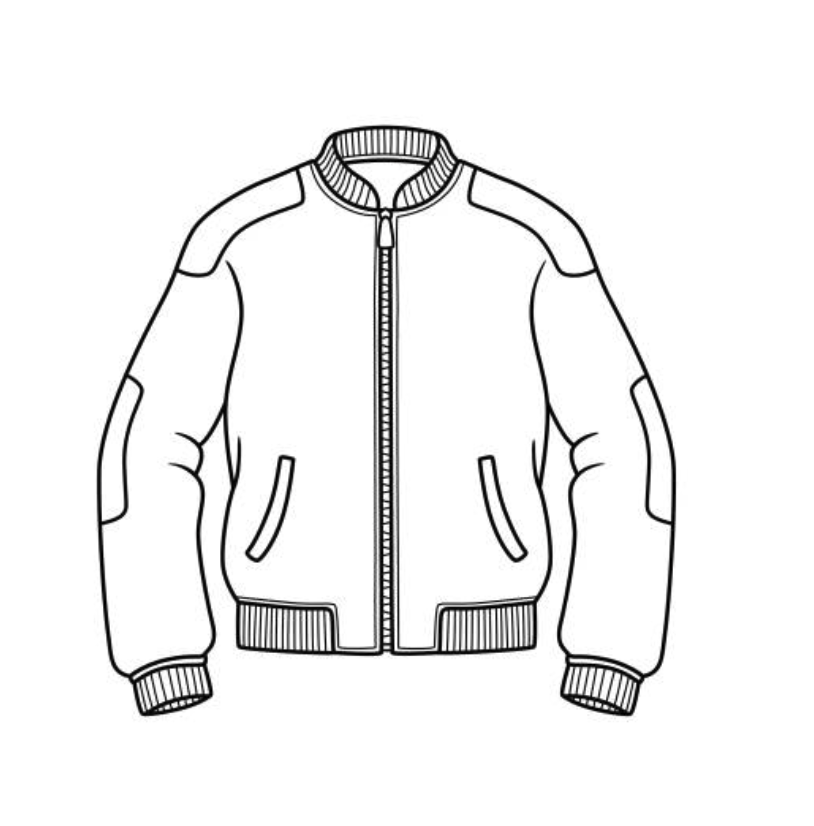
\includegraphics[width=2cm]{Screenshot_2025-03-09_at_22.37.32.png} & White & 7890 & 1 \\[1cm]
    \hline
    Size Label & Woven size indicator & 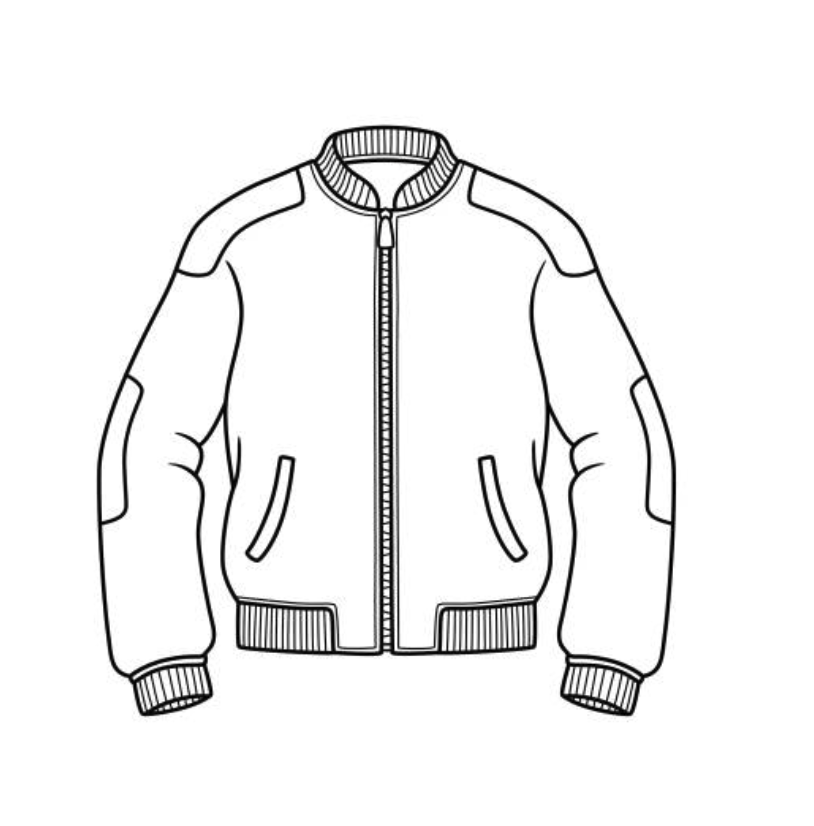
\includegraphics[width=2cm]{Screenshot_2025-03-09_at_22.37.32.png} & White & 1357 & 1 \\[1cm]
    \hline
    Hang Tag & Cardboard with logo & 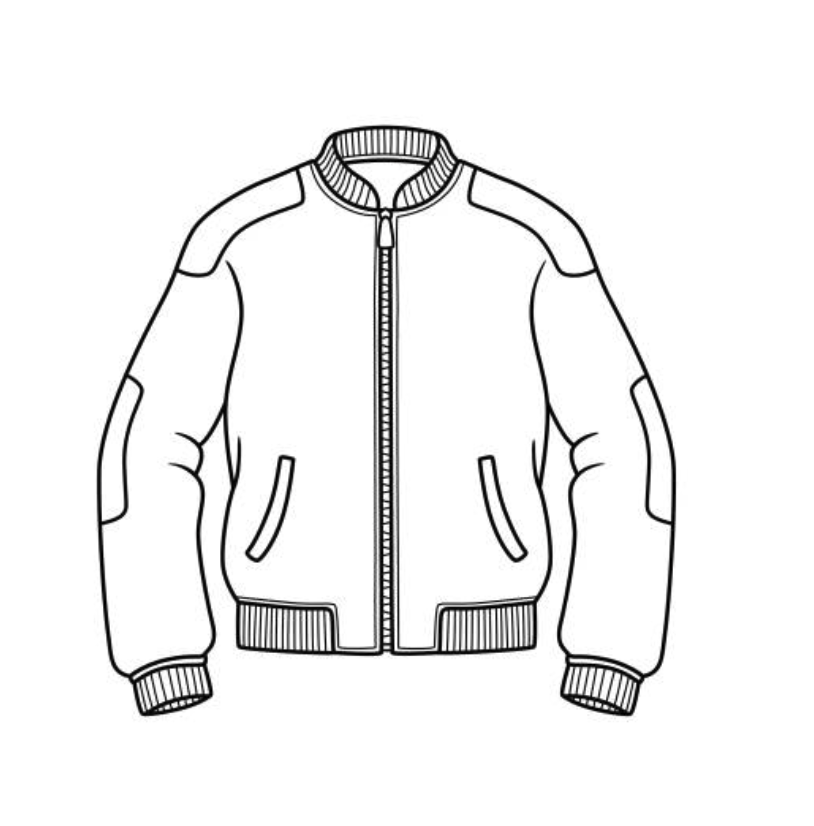
\includegraphics[width=2cm]{Screenshot_2025-03-09_at_22.37.32.png} & Black & 2468 & 1 \\[1cm]
    \hline
  \end{tabular}%
  }
\end{table}

\vspace{0.8cm}
\techsection{Packaging}
\begin{table}[H]
  \centering
  \resizebox{\linewidth}{!}{%
  \begin{tabular}{|p{2.5cm}|p{4cm}|p{3cm}|p{2.5cm}|p{2cm}|p{2.5cm}|}
    \hline
    \rowcolor{tableheader}
    \textbf{Item} & \textbf{Description} & \textbf{Image} & \textbf{Color} & \textbf{Code} & \textbf{Quantity} \\
    \hline
    Polybag & Clear plastic & 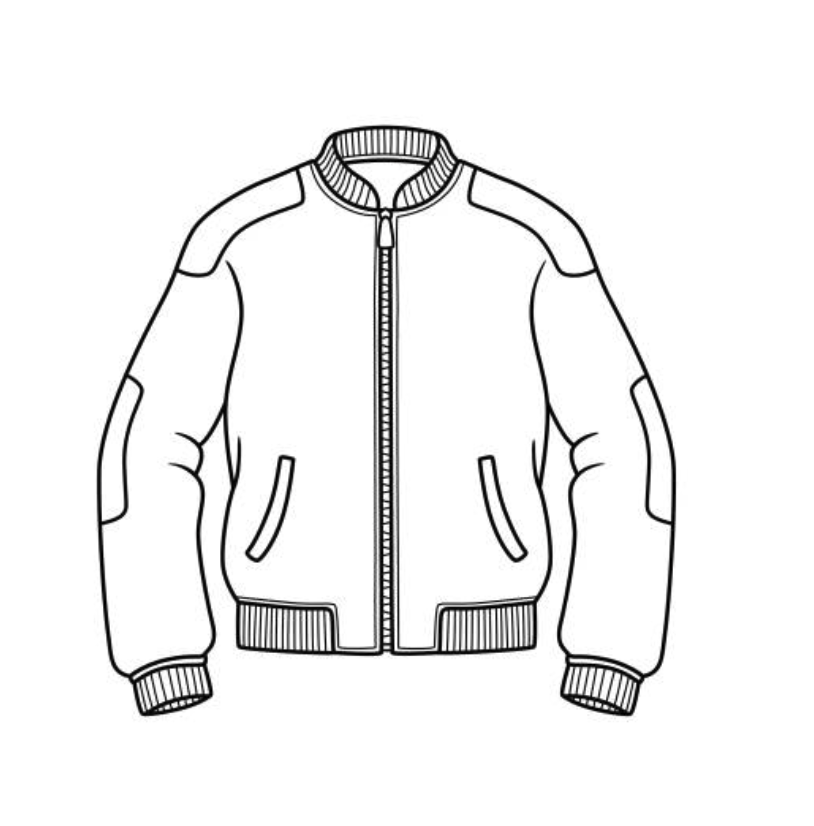
\includegraphics[width=2cm]{Screenshot_2025-03-09_at_22.37.32.png} & Transparent & 1010 & 1 \\[1cm]
    \hline
    Folding Instructions & Printed card & 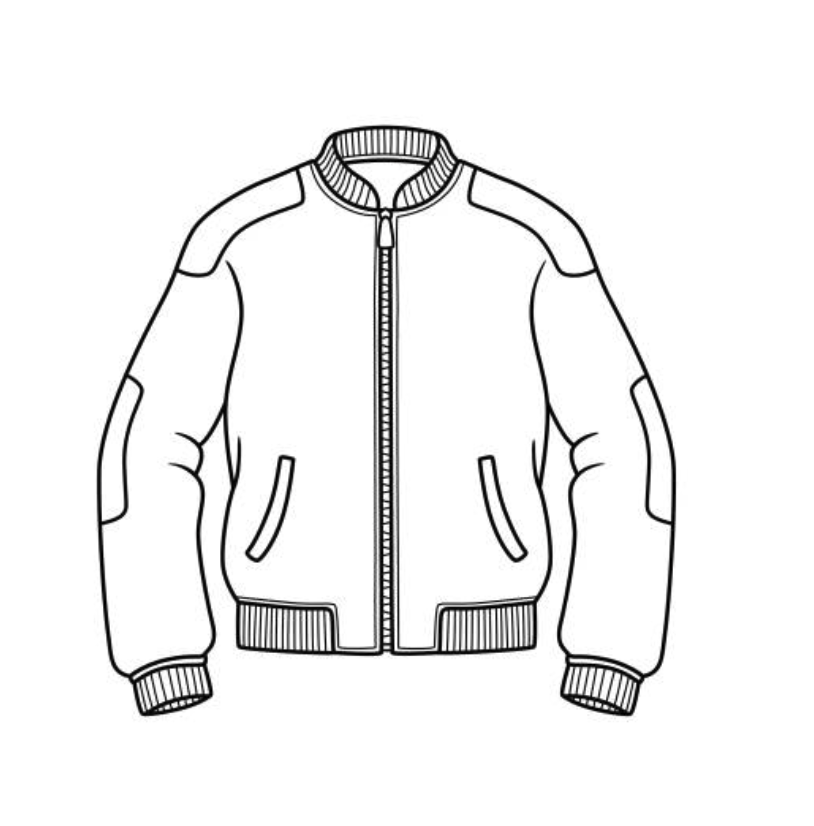
\includegraphics[width=2cm]{Screenshot_2025-03-09_at_22.37.32.png} & White & 2020 & 1 \\[1cm]
    \hline
  \end{tabular}%
  }
\end{table}

%%%%%%%%%%%%%%%%%%%%%%%%%%%%%%%%%%%%%%%%%%%%
% Page 11: Legal Disclaimers
%%%%%%%%%%%%%%%%%%%%%%%%%%%%%%%%%%%%%%%%%%%%

\newpage
\techsection{CONFIDENTIALITY \& USAGE DISCLAIMER}
\begin{tcolorbox}[
  enhanced,
  colback=white,
  colframe=bordergray,
  width=\textwidth,
  arc=0mm,
  boxrule=0.5mm
]
This Tech Pack is the exclusive intellectual property of \CompanyName\ and is intended strictly for internal use and its authorized manufacturing, production, and supply chain partners. The contents of this document—including, but not limited to, designs, specifications, measurements, materials, and construction details—are proprietary and confidential information owned solely by \CompanyName.

Any unauthorized reproduction, distribution, modification, or disclosure of this document, whether in part or in full, is strictly prohibited and constitutes a violation of intellectual property rights. This Tech Pack must not be shared with any third parties, subcontractors, or competitors without prior written consent from \CompanyName. Any misuse or misrepresentation of this document, its contents, or its designs may result in immediate legal action and severe financial penalties.

By accessing or utilizing this Tech Pack, the recipient explicitly agrees to:
\begin{itemize}[itemsep=0.3cm]
  \item Use this document exclusively for the production of goods for \CompanyName.
  \item Not share, disclose, or replicate the information with any unauthorized entity or individual.
  \item Return or destroy any copies of this document upon request by \CompanyName.
  \item Ensure all employees, contractors, and affiliated personnel comply with the confidentiality requirements stated herein.
\end{itemize}

Failure to adhere to these terms will be considered a breach of confidentiality and intellectual property laws, and \CompanyName\ reserves the right to seek legal remedies, financial compensation, and termination of any existing contracts or agreements.

For any clarifications, approvals, or permissions regarding this Tech Pack, please contact \CompanyName\ directly.
\end{tcolorbox}

\vspace{0.8cm}
\techsection{LEGAL NOTICE}
\begin{tcolorbox}[
  enhanced,
  colback=white,
  colframe=bordergray,
  width=\textwidth,
  arc=0mm,
  boxrule=0.5mm
]
This document and all information contained within are protected under applicable copyright,
trademark, and intellectual property laws. Unauthorized use, replication, or distribution
may result in civil and/or criminal prosecution under national and international laws.

\textcopyright\
\ \CompanyName\ \the\year. All Rights Reserved.
Unauthorized use is punishable by law.
\end{tcolorbox}

\end{document}
```